\documentclass[aspectratio=169]{beamer}
\usepackage{tikz}

\usepackage{amssymb,amsmath}
\usepackage{graphicx}
\usepackage{url}
\usepackage{color}
\usepackage{relsize}		% For \smaller
\usepackage{url}			% For \url
\usepackage{epstopdf}	% Included EPS files automatically converted to PDF to include with pdflatex
\usepackage{pagenote}[continuous,page]

%For MindMaps
% \usepackage{tikz}%
% \usetikzlibrary{mindmap,trees,arrows}%

%%% Color Definitions %%%%%%%%%%%%%%%%%%%%%%%%%%%%%%%%%%%%%%%%%%%%%%%%%%%%%%%%%
%\definecolor{bordercol}{RGB}{40,40,40}
%\definecolor{headercol1}{RGB}{186,215,230}
%\definecolor{headercol2}{RGB}{80,80,80}
%\definecolor{headerfontcol}{RGB}{0,0,0}
%\definecolor{boxcolor}{RGB}{186,215,230}

%%% Save space in lists. Use this after the opening of the list %%%%%%%%%%%%%%%%
%\newcommand{\compresslist}{
%	\setlength{\itemsep}{1pt}
%	\setlength{\parskip}{0pt}
%	\setlength{\parsep}{0pt}
%}

%\setbeameroption{show notes on top}

% You should run 'pdflatex' TWICE, because of TOC issues.

% Rename this file.  A common temptation for first-time slide makers
% is to name it something like ``my_talk.tex'' or
% ``john_doe_talk.tex'' or even ``discrete_math_seminar_talk.tex''.
% You really won't like any of these titles the second time you give a
% talk.  Try naming your tex file something more descriptive, like
% ``riemann_hypothesis_short_proof_talk.tex''.  Even better (in case
% you recycle 99% of a talk, but still want to change a little, and
% retain copies of each), how about
% ``riemann_hypothesis_short_proof_MIT-Colloquium.2000-01-01.tex''?

\mode<presentation>
{
  % A tip: pick a theme you like first, and THEN modify the color theme, and then add math content.
  % Warsaw is the theme selected by default in Beamer's installation sample files.

  %%%%%%%%%%%%%%%%%%%%%%%%%%%% THEME
  %\usetheme{Madrid}		% No subsection
  \usetheme{AnnArbor}  % Subsection on top, no color


  %\usetheme{Antibes}
  %\usetheme{Bergen}
  %\usetheme{Berkeley}		% bem bacana - menu esquerdo
  %\usetheme{Berlin}
  %\usetheme{Boadilla}
  %\usetheme{boxes}
  %\usetheme{CambridgeUS}		% bem bacana - menu superior
  %\usetheme{Copenhagen}
  %\usetheme{Darmstadt}
  %\usetheme{default}
  %\usetheme{Dresden}
  %\usetheme{Frankfurt}
  %\usetheme{Goettingen}
  %\usetheme{Hannover}		% bem bacana - menu esquerdo
  %\usetheme{Ilmenau}
  %\usetheme{JuanLesPins}
  %\usetheme{Luebeck}
  %\usetheme{Malmoe}
  %\usetheme{Marburg}		% bem bacana - menu direito
  %\usetheme{Montpellier}
  %\usetheme{PaloAlto}		% bem bacana - menu esquerdo
  %\usetheme{Pittsburgh}
  %\usetheme{Rochester}		%bacana
  %\usetheme{Singapore}
  %\usetheme{Szeged}
  %\usetheme{Warsaw}

  %%%%%%%%%%%%%%%%%%%%%%%%%%%% COLOR THEME
  %\usecolortheme{default}		% branco, azul clarinho
  \usecolortheme{crane}		% Very yellow (ok)

  %\usecolortheme{albatross}		% azul escuro, massa
  %\usecolortheme{beetle}		% cinza, menu azul
  %\usecolortheme{dolphin}		% azul e branco, legal
  %\usecolortheme{dove}			% cinza e branco, feio
  %\usecolortheme{fly}			% todo cinza, horrível
  %\usecolortheme{lily}			% parece o default
  %\usecolortheme{orchid}		% azul e branco, ok
  %\usecolortheme{rose}			% branco e violeta-claro, bonito
  %\usecolortheme{seagull}		% cinza, feio
  %\usecolortheme{seahorse}		% nhé, meio feio
  %\usecolortheme{sidebartab}		% Azul, branco, destaque na tab, interessante
  %\usecolortheme{structure}		% bichado
  %\usecolortheme{whale}		% Azul e branco, bem bonito

  %%%%%%%%%%%%%%%%%%%%%%%%%%%% OUTER THEME
  \useoutertheme{default}
  %\useoutertheme{infolines}
  %\useoutertheme{miniframes}
  %\useoutertheme{shadow}
  %\useoutertheme{sidebar}
  %\useoutertheme{smoothbars}
  %\useoutertheme{smoothtree}
  %\useoutertheme{split}
  %\useoutertheme{tree}

  %%%%%%%%%%%%%%%%%%%%%%%%%%%% INNER THEME
  \useinnertheme{circles}
  %\useinnertheme{default}
  %\useinnertheme{inmargin}
  %\useinnertheme{rectangles}
  %\useinnertheme{rounded}

  %%%%%%%%%%%%%%%%%%%%%%%%%%%%%%%%%%%

  \setbeamercovered{invisible} % or whatever (possibly just delete it)
  % To change behavior of \uncover from graying out to totally
  % invisible, can change \setbeamercovered to invisible instead of
  % transparent. apparently there are also 'dynamic' modes that make
  % the amount of graying depend on how long it'll take until the
  % thing is uncovered.

}


% Get rid of nav bar
\beamertemplatenavigationsymbolsempty

% Use short top
%\usepackage[headheight=12pt,footheight=12pt]{beamerthemeboxes}
%\addheadboxtemplate{\color{black}}{
%\hskip0.5cm
%\color{white}
%\insertshortauthor \ \ \ \
%\insertframenumber \ \ \ \ \ \ \
%\insertsection \ \ \ \ \ \ \ \ \ \ \ \ \ \ \ \ \  \insertsubsection
%\hskip0.5cm}
%\addheadboxtemplate{\color{black}}{
%\color{white}
%\ \ \ \
%\insertsection
%}
%\addheadboxtemplate{\color{black}}{
%\color{white}
%\ \ \ \
%\insertsubsection
%}

% Insert frame number at bottom of the page.
% \usefoottemplate{\hfil\tiny{\color{black!90}\insertframenumber}}

%% makes the ppagenote command for figure references at the end.

\usepackage[english]{babel}
%qq\usepackage[latin1]{inputenc}
\usepackage{CJKutf8}
\usepackage{subfigure}

\usepackage{times}
\usepackage[T1]{fontenc}

\makepagenote
\renewcommand{\notenumintext}[1]{}
\newcommand{\ppagenote}[1]{\pagenote[Page \insertframenumber]{#1}}

\title[Programming Challenges]{GB20602 - Programming Challenges}
\author[Claus Aranha]{Claus Aranha\\{\footnotesize caranha@cs.tsukuba.ac.jp}}
\institute[U. Tsukuba]{University of Tsukuba, Department of Computer Sciences}


\subtitle[Week 4: Dynamic Programming]{Week 4 - Dynamic Programming}
\date[]{{\smaller(last updated: \today)}}

\begin{document}
\begin{CJK}{UTF8}{ipxm}

\begin{frame}
\maketitle
\vfill

\hfill Version 2021.1
\end{frame}

\subsection{Outline}

\begin{frame}
  \frametitle{Review of Last Week}
  \begin{itemize}
  \item {\bf Search Algorithms} are defined by the systematic testing of the {\bf Search Space} of a problem;\bigskip

  \item We studied three types of Search Algorithms:
    \begin{itemize}
    \item Complete Search
    \item Divide and Conquer
    \item Greedy Search
    \end{itemize}
  \end{itemize}
  \bigskip

  \begin{block}{}
    This week we introduce a fourth search algorithm: {\bf Dynamic Programming}.
    \medskip

    Dynamic Programming is one of the most used algorithm in programming competitions.\medskip

    The basic idea is that we can exchange "computation time" for "memory".
  \end{block}
\end{frame}


\section{Introduction to Dynamic Programming}

\begin{frame}
  \begin{center}
    {\bf Part I -- Introduction}
  \end{center}
\end{frame}

\subsection{Definitions}
\begin{frame}
  \frametitle{What is Dynamic Programming (DP)?}

  \structure{DP} is a \structure{Search Algorithm} based on the idea of {\bf Storing Partial Solutions in Memory}.

  \bigskip

  \begin{block}{Basic Idea of DP}
    \begin{itemize}
      \item Create a {\bf DP table}. The dimensions are the parameters of a recursive function that generates the solution to the problem; \bigskip

      \item First fill in the table with the starting conditions;\bigskip

      \item Next use the recursive function (or a for loop) to fill the rest of the table;\bigskip

      \item Find the answer;
    \end{itemize}
  \end{block}
\end{frame}

\begin{frame}{What is Dynamic Programming (DP)?}{Characteristics}

  \begin{block}{If a problem requires {\bf optimization} or {\bf counting}, then it "smells of DP"}

    \begin{itemize}
    \item ``Count the number of solutions...''
    \item ``Find the minimum cost...''
    \item ``Find the maximum length...''
    \end{itemize}
  \end{block}

  \begin{exampleblock}{What is the running cost of DP?}
    The algorithm evaluates each element of the DP table.\medskip

    So the cost of a DP algorithm is proportional to the {\bf size of the DP table.}
  \end{exampleblock}

  You can prove a DP algorithm to be correct using {\bf Proof by Induction}.
\end{frame}

\subsection{Example Problem I}

\begin{frame}{Problem Example: Wedding Shopping}{Problem Summary}

  We have to choose a set of items to buy, within a maximum budget $M$.

    \begin{columns}
      \column{0.7\textwidth}
    \begin{itemize}
      \item There are $C$ classes of items;
      \item Each class has $K_c$ options;
      \item Each option ($K_{c,i}$) has a different cost;
      \bigskip

      \item Buy one item from each Class;
      \item Maximize the total cost, but {\bf do not} exceed the budget $M$;
      \bigskip

      \item Limits: $M \leq 200$, $1 < C \leq 20$, $0 < K_c \leq 20$
    \end{itemize}

      \column{0.3\textwidth}
      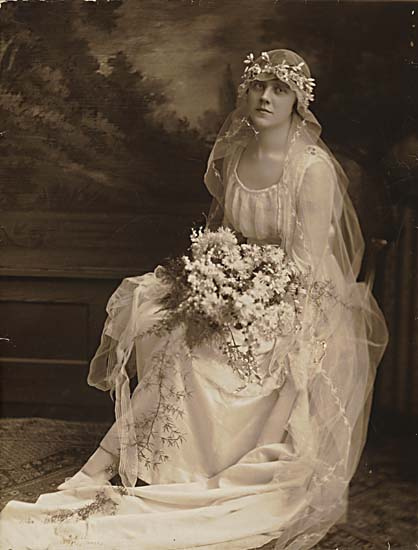
\includegraphics[width=.8\textwidth]{../img/weddingdress}\\
    \end{columns}\bigskip

    {\bf QUIZ: How many possible combinations exist in the largest case?}

    \ppagenote{Wedding Dress Image CC-By-2.0 by \url{https://www.flickr.com/photos/vancouver125/5634967507}}
\end{frame}

\begin{frame}{Problem Example: Wedding Shopping}{Solution Example}
  \begin{block}{Sample case 1: $C=3, K_c = \{3,2,4\}$}
  \begin{tabular}{|c|cccc|}
    Class & 1 & 2 & 3 & 4\\
    \hline
    $K_0$ & 6 & 4 & 8 & \\
    $K_1$ & 5 & 10 & & \\
    $K_2$ & 1 & 5 & 3 & 5\\
  \end{tabular}
  \end{block}
  \medskip

  If the budget is $M=20$, the answer is $19$. Three ways to reach this answer:
  \begin{itemize}
    \item $8(K_{0,2})+10(K_{1,1})+1(K_{2,0})$
    \item $6(K_{0,0})+10(K_{1,1})+3(K_{2,2})$
    \item $4(K_{0,1})+10(K_{1,1})+5(K_{2,1} \text{ or } K_{2,3})$
  \end{itemize}
  \bigskip

  However, if the budget is $M=9$, There is no solution for the problem.\\
  Because the minimum possible cost is $10$, or $4(K_{0,1})+5(K_{1,0})+1(K_{2,0})$
\end{frame}

\begin{frame}[fragile]{Problem Example: Wedding Shopping}{Complete Search Solution}
  This is a {\bf Search problem}: one solution is defined as "one choice from each class".\medskip

  Unfortunately, a Greedy Algorithm will not work in this algorith. So first let's describe a full recursive search:


{\smaller
\begin{verbatim}
shop(m,g):                 // Recursive function. Returns the money used
                           // after start buying from category "g"
  if (m > M) return -1     // End case -- we spend more money than the budget.
  if (g == C) return m     // End case -- we bought all categories.
                           //             Return the total money used.
  for each i in Kc:
    totals[i] = shop(m + price[g][i], g+1) // try buying item i at category g.

  return max(totals)       // Return the value of the best item.

shop(0,0)                  // Start condition: buying from category 0
                           // No money used.
\end{verbatim}
}
\end{frame}

\begin{frame}{Problem Example: Wedding Shopping}{Complete Search Solution -- Time Limited Exceeded :-(}

  In the worst case, there are a total of $20^{20}$ possible choices. So the complete solution will not solve this problem...\bigskip

  \begin{block}{Problem: Too many overlapping subproblems}
    \medskip
    \begin{columns}[T]
      \column{0.4\textwidth}
      \hspace{.5cm}\begin{tabular}{|c|cccc|}
        Class & 1 & 2 & 3 & 4\\
        \hline
        0 & 6 & 4 & 8 & 12\\
        1 & 4 & 6 & 6 & 2\\
        2 & 1 & 5 & 1 & 5\\
        3 & 2 & 4 & 6 & 2\\
      \end{tabular}

      \column{0.6\textwidth}
      Consider: How many times the program in the last slide will call "\emph{shop(10,2)}?"\medskip

      \begin{itemize}
        \item shop(0,0) $\to$ shop(6,1) $\to$ shop(10,2)
        \item shop(0,0) $\to$ shop(4,1) $\to$ shop(10,2) x2
        \item shop(0,0) $\to$ shop(8,1) $\to$ shop(10,2)
      \end{itemize}\medskip

      Every time \emph{shop(10,2)} is called, {\bf the return value is always the same.}
    \end{columns}
  \end{block}
\end{frame}


\begin{frame}
  \frametitle{Wedding Shopping -- the DP approach}

  When a problem has this characteristic ({\bf repeated sub-structures}), it is a strong hint that DP is a good solution.
  \bigskip

  First, we create a {\bf DP table} using the parameters of the "shop(m,g)" function.\bigskip

  Remember: "shop(m,g)" always returns the same value.

  \begin{block}{How big is the table?}
    The table stores all possible calls of \emph{shop(m,g)}, so the table size is $|M| \times |C|$.
    \bigskip

    Remember that $0 \leq M \leq 200$ and $1 < C \leq 20$, so our table has \alert{$201*20=4020$ states}.
  \end{block}
  \smallskip

  That is a very small number! This algorithm will be FAST, compared to $20^{20}$.
\end{frame}

\begin{frame}{Wedding Shopping -- the DP approach}{How to fill the table?}

  There are two main approaches for filling the {\bf DP table}:
  \bigskip

  \begin{itemize}
  \item {\bf Top-down approach}: \\Use the DP table as a "memory" table.\\
  Every time we call the function: If the result is in the table, use that result. If not, calculate and store in the table. Very common with {\bf "recursive functions"}.
  \vfill

  \item {\bf Bottom-up approach}: \\
  First we complete the starting values of the table. Then we fill other values based on the starting values. Very common with {\bf "for loops"}.
  \end{itemize}
\end{frame}

%%%%%%%%%%%%%%
%% Solution: Dynamic Programming
% Programming here is not "code", but a "tabular method" (table method)

%% DP us normally used when
% Program has optimal sub structure:
%   The optimal solution to the problem contain optimal solutions to sub problems
%   - "similar" to the requirement of greedy
%   - If you can make a complete search recurrent (recursive), then you have this
% The subproblems are overlapping
%   - The number of _Distinct_ subproblems is small, but they are computed repeatedly
%   - Different from divide and conquer, in DC the sub problems are distinct
%%%%%%%%%%%%%
\subsection{DP Programming Examples}

\begin{frame}[fragile]{Wedding Shopping -- the DP approach}
  {Using Top-down DP -- very easy to program!}

\begin{block}{}
{\smaller
\begin{verbatim}
memset(table, -2, sizeof(table))  //-1 = "no result", -2 = "not visited"

shop(m,g):
  if (m > M) return -1                      // End States are the same;
  if (g == C) return m
  if (table[m][g] != -2) return table[m][g] // Check if the result is in memory

  for each i in Kc:                         // Calculate as before;
    totals[i] = shop(m + price[g][i], g+1)

  table[m][g] = max(totals)                 // Store new result in table;
  return table[m][g]

shop(0,0)                                   // That's the only change!
\end{verbatim}}
\end{block}
\end{frame}

%%% TODO: Add how to print after the bottom up DP
%% What if you need to print the result (maybe not add this?)
% for each level, you check the lower level to see which one matches the current state
% See slide 16 for details

\begin{frame}{Wedding Shopping -- The DP approach}{Using bottom-up DP}
  Algorithm:
  \begin{itemize}
  \item Prepare a table with the problem states (same table as top-down);
  \item Choose the initial states of the table;
  \item Mark the initial states as "unprocessed";
  \item {\bf (Loop)} For each unprocessed value, calculate its value, and add the new unprocessed values.
  \end{itemize}

  \vfill

  The main difficulties in bottom-up DP are:
  \begin{itemize}
    \item To find the initial states;
    \item To choose the processing function;
  \end{itemize}
  After that, it is just a big "for loop".
\end{frame}

\begin{frame}{Wedding Shopping -- Bottom-up DP}{One possible solution}

  Example: M=10, \alert<2>{$K_0=\{2,4\}$}, \alert<3>{$K_1=\{4,6\}$}, \alert<4>{$K_2=\{1,3,2,1\}$}
  \bigskip

  \begin{tabular}{|c||c|c|c|c|c|c|c|c|c|c|c|c|}
    \hline
    M & 0 & 1 & 2 & 3 & 4 & 5 & 6 & 7 & 8 & 9 & 10\\
    \hline
    $g=0$ & X & & & & & & & & & & \\
    $g=1$ & & & \only<2->{X} & & \only<2->{X} & & & & & & \\
    $g=2$ & & & & & & & \only<3->{X} & & \only<3->{X} & & \only<3->{X}\\
    $g=3$ & & & & & & & & \only<4->{X} & \only<4->{X} & \only<4->{X} & \only<4->{X}\\
    \hline
  \end{tabular}

  \begin{itemize}
  \item {\bf Start state}: We use no money, so mark $T(0,0)$ as "unprocessed".
  \item {\bf Transition Function} (from category c to category c+1):
    \begin{itemize}
      \item Loop on money: $i = 0\to m$
      \item If $T(g,i)$ is marked as "unprocessed"
      \begin{itemize}
        \item Loop: $j = 0\to |K_c|$
        \item Mark $T(s+1,i+K_{c,j})$ as "unprocessed"
      \end{itemize}
    \end{itemize}
  \item {\bf Solution}: The solution is the maximum column marked when $g = C$
  \end{itemize}
\end{frame}

\begin{frame}[fragile]{Wedding Shopping -- Bottom-up DP}

  Example: M=10, $K_0=\{2,4\}$, $K_1=\{4,6\}$, $K_2=\{1,3,2,1\}$
  \bigskip

  \begin{tabular}{|c||c|c|c|c|c|c|c|c|c|c|c|c|}
    \hline
    M & 0 & 1 & 2 & 3 & 4 & 5 & 6 & 7 & 8 & 9 & 10\\
    \hline
    $s=0$ & X & & & & & & & & & & \\
    $s=1$ & & & X & & X & & & & & & \\
    $s=2$ & & & & & & & X & & X & & X\\
    $s=3$ & & & & & & & & X & X & X & X\\
    \hline
  \end{tabular}
  {\smaller
  \begin{block}{}
\begin{verbatim}
memset(table,0,sizeof(table))
table[0][0] = 1

for g in (0 to C-1)
  for i in (0 to M-1):
    if table[g][i] == 1:
       for k in (0 to K[g]-1):
          table[g + 1][i + cost[g][k]] = 1 // Don't forget out of bounds check!
\end{verbatim}
  \end{block}}
\end{frame}

\begin{frame}
  \frametitle{DP: Top-down or Bottom-up?}

  \begin{block}{Top-Down}
    {\bf Pros:} Easy to implement, just add memory to a recursive search. Only computes the visited states of the DP table. \medskip

    {\bf Cons:} Overhead of recursive function. Hard to reduce the size of the DP table.
  \end{block}

  \begin{block}{Bottom-Up}
    {\bf Pros:} Faster if you will visit the entire DP table anyway. It is possible to save memory by discarding old rows.\medskip

    {\bf Cons:} Harder to think the algorithm. If the DP table is sparse, the loop will visit every state.
  \end{block}
\end{frame}

\subsection{DP Example 2}

\begin{frame}{Finding the Decision Set with DP}

  In the example we studied, the program only returns the total money used.\bigskip

  In some problems, we also need to output the {\bf optimal solution} (for example, optimal path). How do we do that?
  \bigskip

  It is not very hard. You need TWO tables:
  \begin{itemize}
    \item Table 1: The DP table (memory table);
    \item Table 2: The "Parent" table, which indicate what was the previous choice.
  \end{itemize}
  \bigskip

  The next example will show the use of the "Parent" table. \bigskip

  \begin{block}{}
    When filling the parent table, be careful about the rules for tie breaking!\\
    (Lexographical order, smallest solution, etc).
  \end{block}
\end{frame}

\begin{frame}{Example 2: Apple Field}
  \begin{block}{}
  {\smaller
  A farmer has an apple field, and a robot to collect the apples. However, the robot can only move {\bf one left} or {\bf one down}. The robot starts at position $(0,0)$, and ends at $(n,n)$.\medskip

  You know how many apples are in each cell. What is the path with maximum apples?
}
  \end{block}

  \begin{center}
    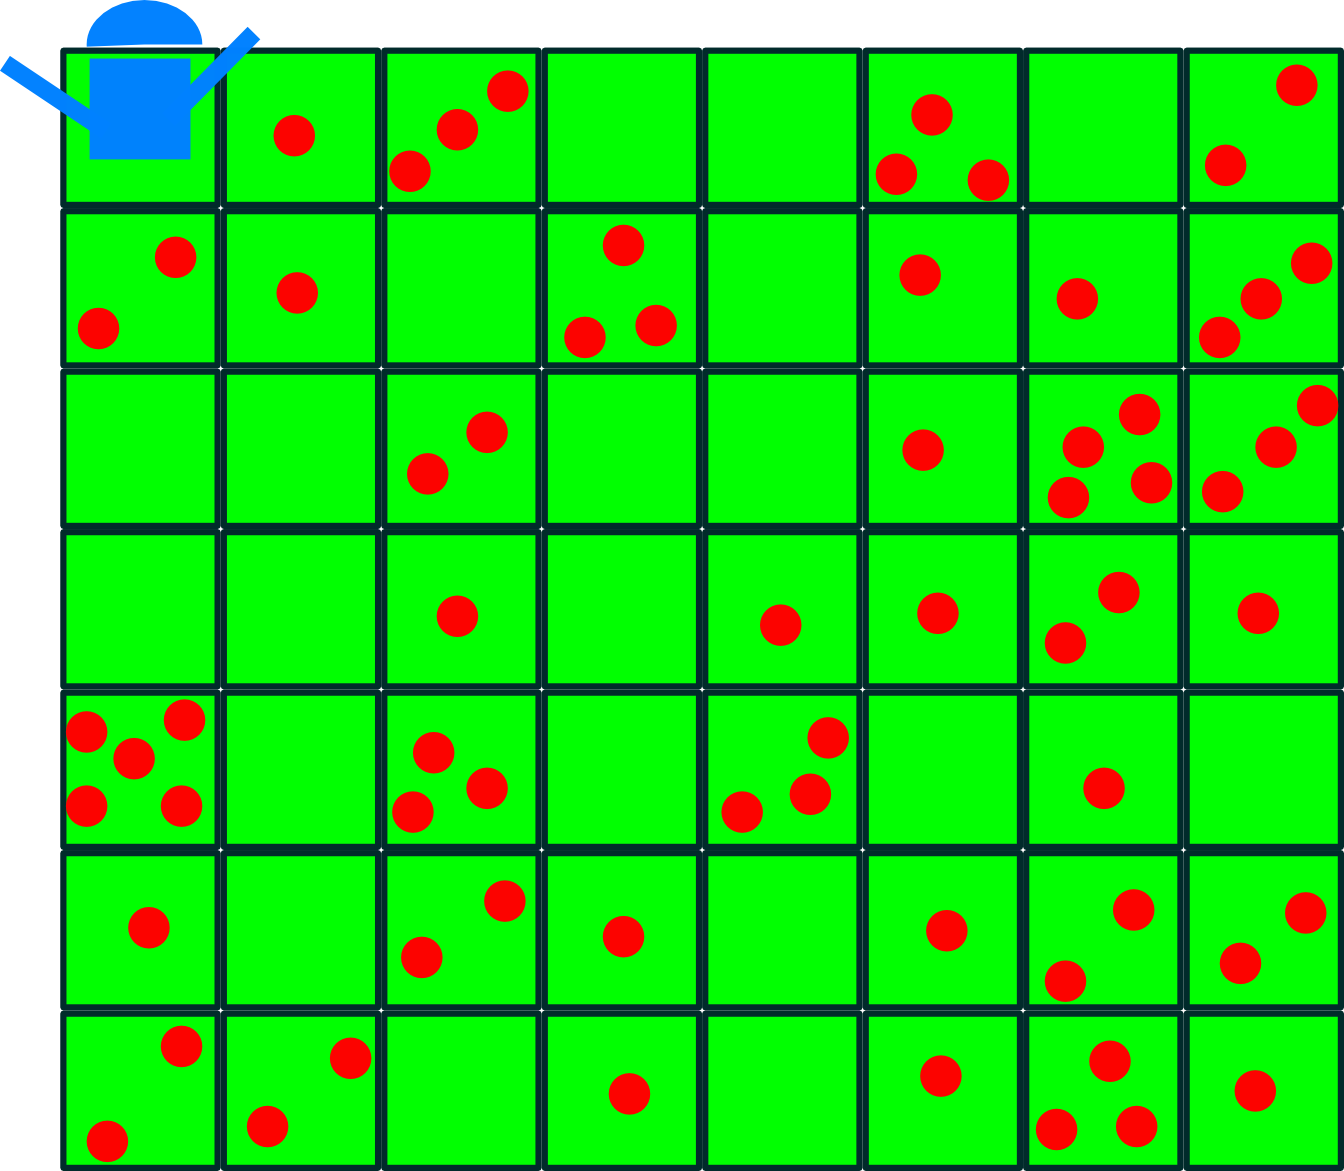
\includegraphics[width=0.4\textwidth]{../img/applefield}
  \end{center}
\end{frame}

\begin{frame}{Example 2: Apple Field}{One Possible Solution (Not maximum)}

  \begin{columns}
    \column{0.5\textwidth}
    L, D, L, L, L, L, L, L, D, D, D, D, L, D
    \column{0.5\textwidth}
    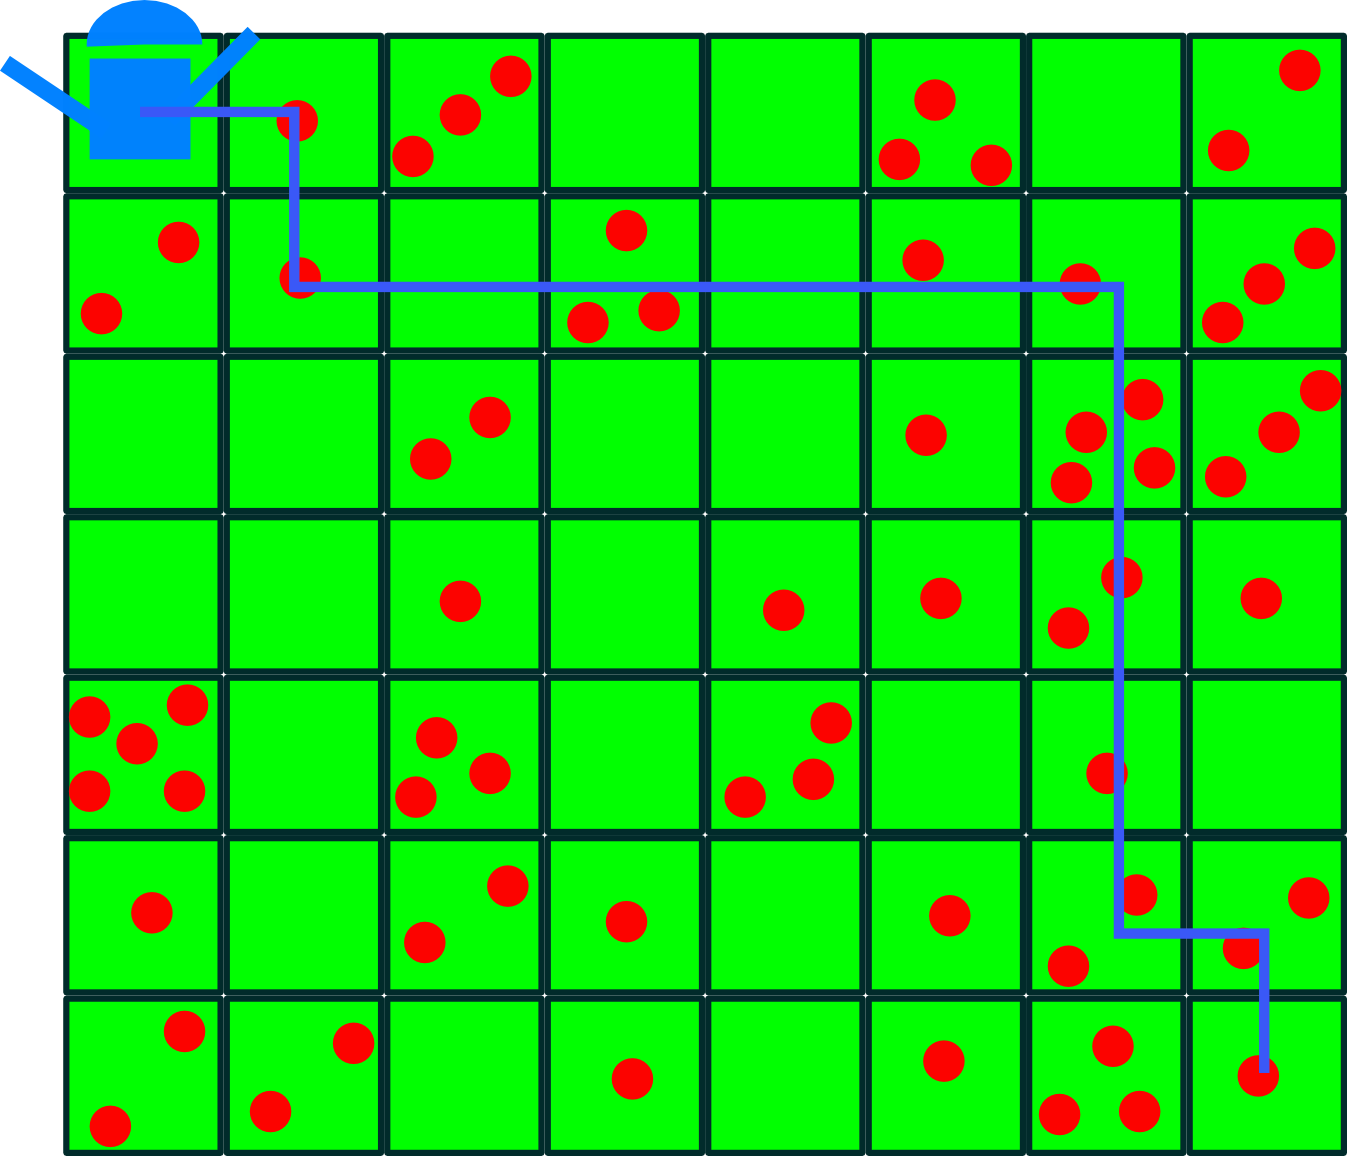
\includegraphics[width=0.9\textwidth]{../img/applefield-solution}
  \end{columns}
\end{frame}

\begin{frame}{Example 2: Apple Field}{Complete Search}

  \begin{block}{}
    How many different paths are possible?
  \end{block}
  \begin{itemize}
    \item A path has $n$ steps left (0), and $n$ steps down (1), in any order.
    \bigskip

    \item A path is a string with size $2n$, $n$ "0"s, and $n$ "1"s.
    \bigskip

    \item Permutation of $2n$ with $n$ "0"s and $n$ "1"s: $\binom{2n}{n} = \frac{(2n)!}{n!n!}$
    \begin{itemize}
      \item Too big for full search!
    \end{itemize}
  \end{itemize}\bigskip

  Like in the "Wedding Shopping" problem, we have {\bf overlapping subproblems}.
  \bigskip

  For example, the optimal path from $(x,y)$ to $(n,n)$ is always the same, regardless of the path from $(0,0)$ to $(x,y)$. So let's try DP!
\end{frame}


\begin{frame}{Example 2: Apple Field}{Bottom-up DP}
  \begin{itemize}
  \item {\bf DP table and Parent table:}
  \begin{itemize}
    \item The DP table is a $n+1\times n+1$ table. At every position, we have the maximum number of apples from $(0,0)\to(x,y)$.
    \item The Parent table is a $n+1\times n+1$ table. At every position, we store the last-1 cell (up or right) of $(0,0)\to(x,y)$.
  \end{itemize}

  \item {\bf Initial Condition:} (DP table only)
  \begin{itemize}
    \item To avoid special treatment of the first row and first column, we include a "boundary" at the top and right of the table. Every cell at the boundary has "0" apples
  \end{itemize}

  \item {\bf Transition:}
  \begin{itemize}
    \item We double loop over the DP table (row $\to$ column, or vice-versa). For every cell $(x,y)$:\\
    $DP[x][y] = \text{apple}[x][y] + \text{max}(DP[x-1][y],DP[x][y-1])$\\
    $\text{Parent}[x][y] = (DP[x-1][y] > DP[x][y-1]?\leftarrow:\uparrow)$
  \end{itemize}
  \end{itemize}
\end{frame}

\begin{frame}[fragile]{Example 2: Apple Field}{Pseudocode}
  {\smaller
  \begin{block}{}
\begin{verbatim}
int apple[m+1][n+1];     // Input Data. Board index is from 1 to n

int DP[m+1][n+1];                      // DP Table
DP[0][0..n+1] and DP[0..m+1][0] = 0;   // Initial states;

int parent[m+1][n+1];               // Parent Table;

for (int i = 1; i < m+1; i++) {
  for (int j = 1; j < n+1; j++) {
    DP[m][n] = apple[m][n] + max(DP[m][n-1], DP[m-1][n]);  // Update DP
    if (DP[m][n-1] > DP[m-1][n]):                          // Update Parent
       parent[m][n] = "left";
    else:
       parent[m][n] = "up";
  }
}
\end{verbatim}
\end{block}
  }
\end{frame}



\begin{frame}[fragile]{Example 2: Apple Field}{Simulating the algorithm}

{\smaller
\begin{verbatim}
DP[m][n] = apple[m][n] + max(DP[m][n-1], DP[m-1][n]);
if (DP[m][n-1] > DP[m-1][n]):
   parent[m][n] = "left";
else:
   parent[m][n] = "up";
 \end{verbatim}}

\begin{columns}
  \column{0.3\textwidth}
  \begin{center}
    Input Table\\
    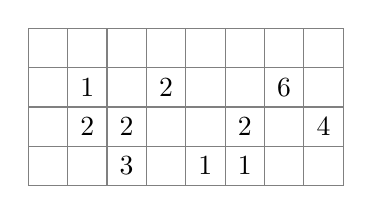
\begin{tikzpicture}
    \draw[step=0.5cm,color=gray] (0,0) grid (4,2);
    %% Row 1
    \node at (.75,1.25) {1};
    \node at (1.75,1.25) {2};
    \node at (3.25,1.25) {6};
    %% Row 2
    \node at (.75,.75) {2};
    \node at (1.25,.75) {2};
    \node at (2.75,.75) {2};
    \node at (3.75,.75) {4};
    %% Row 3
    \node at (1.25,.25) {3};
    \node at (2.25,.25) {1};
    \node at (2.75,.25) {1};
    \end{tikzpicture}
  \end{center}

  \column{0.3\textwidth}
  \begin{center}
  DP Table\\
    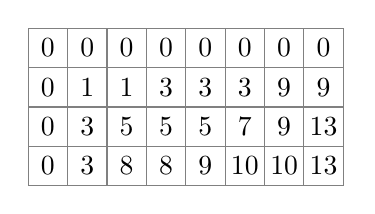
\begin{tikzpicture}
    \draw[step=0.5cm,color=gray] (0,0) grid (4,2);
    \node at (.25,.25) {0};
    \node at (.25,.75) {0};
    \node at (.25,1.25) {0};
    \node at (.25,1.75) {0};
    %
    \node at (.75,1.75) {0};
    \node at (1.25,1.75) {0};
    \node at (1.75,1.75) {0};
    \node at (2.25,1.75) {0};
    \node at (2.75,1.75) {0};
    \node at (3.25,1.75) {0};
    \node at (3.75,1.75) {0};
    %
    \node<2-> at (.75,1.25) {1};
    \node<3-> at (1.25,1.25) {1};
    \node<4-> at (1.75,1.25) {3};
    \node<5-> at (2.25,1.25) {3};
    \node<5-> at (2.75,1.25) {3};
    \node<6-> at (3.25,1.25) {9};
    \node<6-> at (3.75,1.25) {9};
    %
    \node<7-> at (.75,.75) {3};
    \node<8-> at (1.25,.75) {5};
    \node<9-> at (1.75,.75) {5};
    \node<9-> at (2.25,.75) {5};
    \node<10-> at (2.75,.75) {7};
    \node<11-> at (3.25,.75) {9};
    \node<12-> at (3.75,.75) {13};
    %
    \node<13-> at (.75,.25) {3};
    \node<13-> at (1.25,.25) {8};
    \node<13-> at (1.75,.25) {8};
    \node<13-> at (2.25,.25) {9};
    \node<13-> at (2.75,.25) {10};
    \node<13-> at (3.25,.25) {10};
    \node<13-> at (3.75,.25) {13};
    \end{tikzpicture}
  \end{center}

  \column{0.3\textwidth}
  \begin{center}
  Parent Table\\
    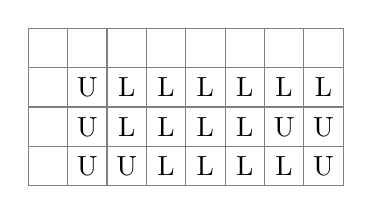
\begin{tikzpicture}
    \draw[step=0.5cm,color=gray] (0,0) grid (4,2);
    %\node at (.25,1.25) {0};
    \node<2-> at (.75,1.25) {U};
    \node<3-> at (1.25,1.25) {L};
    \node<4-> at (1.75,1.25) {L};
    \node<5-> at (2.25,1.25) {L};
    \node<5-> at (2.75,1.25) {L};
    \node<6-> at (3.25,1.25) {L};
    \node<6-> at (3.75,1.25) {L};
    %
    \node<7-> at (.75,.75) {U};
    \node<8-> at (1.25,.75) {L};
    \node<9-> at (1.75,.75) {L};
    \node<9-> at (2.25,.75) {L};
    \node<10-> at (2.75,.75) {L};
    \node<11-> at (3.25,.75) {U};
    \node<12-> at (3.75,.75) {U};
    %
    \node<13-> at (.75,.25) {U};
    \node<13-> at (1.25,.25) {U};
    \node<13-> at (1.75,.25) {L};
    \node<13-> at (2.25,.25) {L};
    \node<13-> at (2.75,.25) {L};
    \node<13-> at (3.25,.25) {L};
    \node<13-> at (3.75,.25) {U};
    \end{tikzpicture}
  \end{center}
\end{columns}

\end{frame}



%\subsection{Flight Planner}
%%%%%%%%%%%%%
%% Example 2 -- UVA 10337 Flight Planner
% 1 Mile Altitude and 1(x100) miles distance
% wind speed map
% fuel cost: Climb +60, hold +30, sink +20 - windspeed wsp[alt][dis]
% Compute min fuel cost from (0,0) to (0,X=4)

%% First guess: Complete search/Backtracking finding path with minimal fuel cost
% Recurrence: minimum of current + climb/Hold/Dive
% Problem: 1000 distance columns: 3^1000 states to search!
% However, there are MANY overlapps: at any column/height, former path does not matter.

%% DP solution
% TOP down: create a 2D table and store computation value of subproblems as they are seen.
% Bottom-up: Start at 0 fuel used. Calculate next column based on where current column can reach
%            Bottom up hint: We just need to store two columns at a time (if only final result is desired)

\section{Classical DP}

\begin{frame}
  \begin{center}
    {\bf Part II -- Classical DP Problems}
  \end{center}
\end{frame}

\begin{frame}{Classical DP Problems}

  There are some classical problems that have well known DP solutions:
  \bigskip

  \begin{itemize}
    \item Max sum;
    \item Max sum 2D;
    \item Longest Increasing Subsequence;
    \item Knapsack Problem;
    \item Coin Change;
  \end{itemize}
  \bigskip

  We will show some examples from each category so you can have a better understanding of the DP philosophy.\bigskip

  {\bf After each problem is explained, try to find the DP table, and the transition function}.
\end{frame}

\subsection{Max Sum}

\begin{frame}[fragile]{The 1D Range Sum Problem}

  Consider an array $A$ containing $N$ integers. We want to find the indexes $i,j, (0 \leq i < j \leq N-1)$ that {\bf maximize} the sum from $A_i$ to $A_j$ ($\sum_{k=i}^{j} A_k$).
  \bigskip

  Example:
\begin{verbatim}
Array A = 1, -3, 20, -2, -5, 10, 5, -4, 6, 47, -30, -3
  Total = 42
RangeSum=        20, -2, -5, 10, 5, -4, 6, 47
  Total = 77
\end{verbatim}
\bigskip

How do you solve this problem?
\end{frame}

\begin{frame}[fragile]{The 1D Range Sum Problem}{Complete Search}
  \begin{block}{    Calculate the range sum for every possible pair $(i,j)$.}

{\smaller
\begin{verbatim}
int minindex, maxindex;
int maxsum = 0;
for (int i = 0; i < n; i++)
   for (int j = 0; i < n; j++)
      int sum = 0;
      for (int k = i; k < j+1; k++)
         sum += k;
      if sum > maxsum:
         maxsum = sum;
         minindex = i; maxindex = j;
\end{verbatim}
}
  \end{block}

  Because of three loops, this approach is $O(n^3)$. For large values of $N$ (for example 10.000), this is not feasible.
\end{frame}

\begin{frame}[fragile]{The 1D Range Sum Problem}{DP Sum Table}
  Note that {\bf sum(i,j) = sum(0,j) - sum(0,i-1)}.\medskip

  Using this fact, we can create a sum table (ST) to calculate the result faster:

  \begin{block}{Using Sum Table -- $O(n^2)$}
{\smaller
\begin{verbatim}
int[] ST; int maxsum = 0; int sum_s = 0; int sum_e = 0; ST[0] = 0;

for (int i = 1; i < N+1; i++) { ST[i] = ST[i-1] + A[i]; } // preprocessing;

for (int i = 1; i < N+1; i++)
  for (int j = i; j < N+1; j++)
    if (ST[j] - ST[i-1] > maxsum) {
      maxsum = ST[j] - ST[i-1];
      sum_s = i; sum_e = j;
    }
\end{verbatim}
}
  \end{block}
\end{frame}

\begin{frame}[fragile]{The 1D Range Sum Problem}{DP Sum Table Simulation}

  Let's visualize how the DP sum table transforms the problem:

{\smaller
\begin{verbatim}
i  =      1,  2,  3,  4,  5,  6,  7,  8,  9, 10, 11, 12
A  =      1, -3, 20, -2, -5, 10,  5, -4,  6, 47,-30, -3
ST = [0], 1, -2, 18, 16, 11, 21, 26, 22, 28, 75, 45, 42

i, j  | ST[j] - ST[i-1] | Total Sum
===================================
1, 12 | 42    - 0       | 42
3, 10 | 75    - (-2)    | 77
6, 8  | 22    - 11      | 11
===================================
\end{verbatim}
}
\bigskip

Can we do even better?
\end{frame}

\begin{frame}[fragile]{The 1D Range Sum Problem}
  {Kadane's Greedy Algorithm -- $O(n)$ mix of Sum Table and Greedy Approach}

  \begin{block}{}
      {\smaller
\begin{verbatim}
A[] = { 4, -5, 4, -3, 4, 4, -4, 4, -5}; // Example
int sum = 0, ans = 0;
for (i in 0:n):
   sum += A[i], ans = max(ans, sum)     // Add to running total
   if (sum < 0) sum = 0;                // If total is negative
                                        // reset the sum;
\end{verbatim}
      }
  \end{block}

\begin{itemize}
\item Basic idea: it is always better to increase the sum,
unless a very large negative sum appears.
\item In that case, it is better to start from zero after the negative sum.
\end{itemize}
\begin{verbatim}
    A  :  4 | -5 | 4 -3  4  4 -4  4 | -5
    Sum:  4 |  0 | 4  1  5  9  5  9 |  4
    ans:  4 |  4 | 4  4  5  9  9  9 |  9
\end{verbatim}
\end{frame}

\subsection{Maximum Sum -- 2D}
\begin{frame}
  \frametitle{Maximum Range Sum -- Now in 2D!}
  \begin{block}{Problem Summary}
    Given an array of positive and negative numbers, find the
    subarray with maximum sum.
  \end{block}
  \begin{center}
    \begin{tabular}{|cccc|}
      \hline
      0 & -2 & -7 & 0\\
      9 & 2 & -6 & 2\\
      -4 & 1 & -4 & 1\\
      -1 & 8 & 0 & -2\\
      \hline
    \end{tabular}
  \end{center}
  \bigskip

  This is the same problem as the previous one, but the second dimention adds some interesting complications.\bigskip

  {\bf QUIZ:}
  \begin{itemize}
    \item What is the cost of a complete search in this case?
    \item How would you write a DP (table and transition)?
  \end{itemize}
\end{frame}

\begin{frame}[fragile]{Maximum Range Sum 2D}{Complete Search}

\begin{block}{}
  The complete search approach needs 6 loops (2 for horizontal axis, 2 for vertical axis, 2 for calculating the sum). So the total complexity is O($n^6$).
\end{block}

\begin{block}{}
{\smaller
\begin{verbatim}
minvalue = -MIN_INT
for i in (0:n):
   for j in (0:n):
      for k in (i:n):
         for l in (j:n):
         sum = 0
         for a in (i:k):
            for b in (j:l):
               sum += A[a,b]
         if sum > minvalue:
            minvalue = sum
\end{verbatim}
}
\end{block}
\end{frame}

\begin{frame}[fragile]{Maximum Range Sum 2D}{Using the Sum Table}

We can use the Sum Table idea from 1D, but be careful about the {\bf Principle of Inclusion-Exclusion}. We subtract the partial sum of two axis, and add back the intersection of that sum.
\bigskip

\begin{columns}
  \column{0.5\textwidth}
  \hfill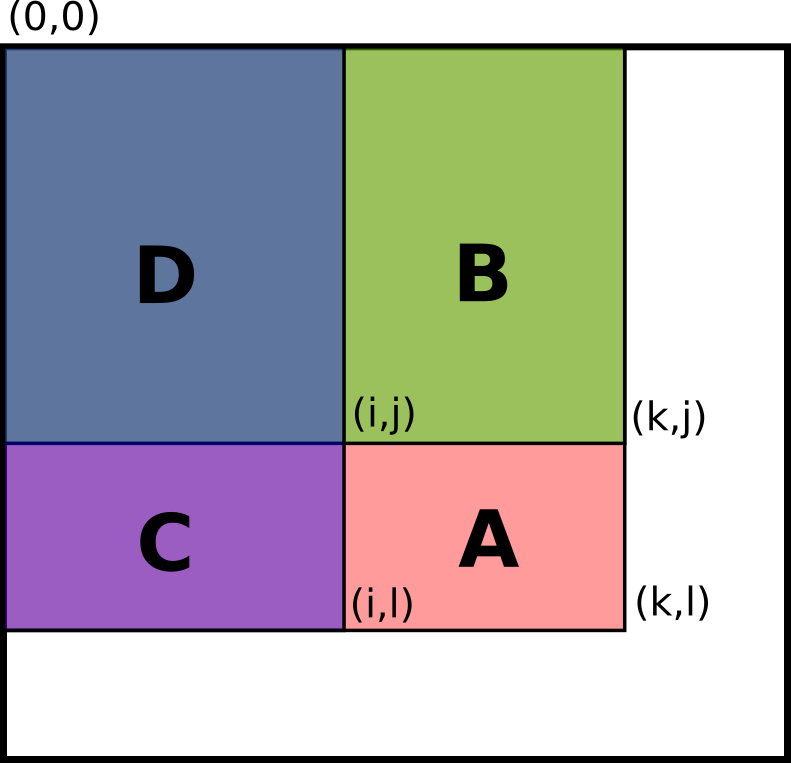
\includegraphics[width=.6\textwidth]{img/inclusion_exclusion}
  \column{0.5\textwidth}
  $A = ABCD - BD - CD + D$
\end{columns}

\end{frame}

\begin{frame}[fragile]{Maximum Range Sum 2D}{2D Sum Table Pseudocode}
\begin{block}{}
{\smaller
\begin{verbatim}
for i in (0:n):                      // Precalculation: Creating ST
   for j in (0:n):
       ST[i][j] = A[i][j]                            // A[i][j] is the input
       if (i > 0) ST[i][j] += ST[i-1][j]
       if (j > 0) ST[i][j] += ST[i][j-1]
       if (i > 0 && j > 0) ST[i][j] -= ST[i-1][j-1]  // Avoid double count

for i,j in (0:n)(0:n):
   for k,l in (i:n)(j:n):
      sum = ST[k][l]                         // Total Sum (0,0)->(k,l)
      if (i > 0) sum -= ST[i-1][l];          // Remove (0,0)->(i-1,l)
      if (j > 0) sum -= ST[k][j-1];          // Remove (0,0)->(k,j-1)
      if (i > 0 && j > 0) sum += A[i-1][j-1] // Add back double remove
      maxsum = max(sum,maxsum)
\end{verbatim}
}
\end{block}

\end{frame}

\subsection{Longest Increasing Subsequence}

\begin{frame}[fragile]{Problem 3: Longest Increasing Subsequence}{Problem Definition}
  \begin{block}{}
    Given a sequence $A$ of integers, find the longest subsequence $S \in A$ where $S_i < S_{i+1} < S_{i+2} < \ldots$.
  \end{block}
  \bigskip

  Example:
\begin{verbatim}
A   = [-7, 10, 9, 2, 3, 8, 8, 1]
S_1 = [-7,        2, 3, 8]          // size 4 -- LIS
S_2 = [-7,     9]                   // size 2
\end{verbatim}
\bigskip

Note that because the subsequence is {\bf not contiguous}, this problem is more difficult than Range Sum.
\bigskip

{\bf QUIZ}: What is the \alert{Complete Search} and \alert{DP approach} (Table and Transition) for this problem?
\end{frame}

\begin{frame}[fragile]
  \frametitle{Complete Search for LIS}

  As other "find the subset" problems, the complete search of LIS can be done by testing all binary strings of size "n". This costs $O(2^n)$.
  \smallskip

  \begin{block}{}
    {\smaller
\begin{verbatim}
// Complete Subset Search using bitmasks
vector<int> S_max; int max_len = 0;// Final Result

for (int i = 0; i < (1<<n); i++) {                // Loop all bitstrings
  vector<int> S; int min = -99999; int len = 0;
  for (int j = 0; j < n; j++) {                   // Creat subset from bitstring
    if ((1<<j)&i) {                               // Add j to subset
      if (A[j] > min) {                           // Test if subset is increasing
        S.push_back(A[j]);
        min = A[j]; len ++;
      } else { break; }                           // Subset not increasing
  } }
  if (len > max_len) { max_len = len; S_max = S; }// Found a longer subset
} }
\end{verbatim}
    }
  \end{block}
\end{frame}

\begin{frame}{DP for Longest Increasing Subsequence}
  As usual, to prepare a DP we decide the {\bf Table} and {\bf Transition}.

  \begin{block}{Transition}
    For every element A[i], that element is either:
    \begin{itemize}
      \item The beginning of a new partial LIS;
      \item Added to the end of an existing partial LIS;
    \end{itemize}
    So for each element, we only need to know which partial LIS this item should be added to.
  \end{block}

  \begin{exampleblock}{Table}
    \begin{itemize}
      \item {\bf Parent}: Indicate the previous element of the longest partial LIS this element is a member of;
      \item {\bf LIS}: Indicate the current size of the longest partial LIS this element is a member of;
    \end{itemize}
  \end{exampleblock}
\end{frame}

\begin{frame}[fragile]{DP for Longest Increasing Subsequence}{Example}
\begin{verbatim}
  A      = [ -7, 10, 9, 2, 3, 8, 8, 1 ]
  parent = [ -1,  0, 0, 0, 3, 4, 4, 0 ]
  LIS    = [  1,  2, 2, 2, 3, 4, 4, 2 ]
\end{verbatim}

\begin{block}{Pseudocode (O($n^2$))}
\begin{verbatim}
LIS[0:n] = 1
parent[0:n] = -1
for i in (1 to n):
   for j in (0 to i): // Try to add to longest LIS
      if (LIS[j] >= LIS[i]) && (A[j] < A[i]):
         LIS[i] = LIS[j] + 1
         parent[i] = j
\end{verbatim}
\end{block}

There is a faster $O(n\log k)$ approach that uses greedy and binary search.
\end{frame}


\subsection{Knapsack problem}
\begin{frame}[fragile]{Classic DP: The 0-1 Knapsack Problem}

  In the 0-1 Knapsack problem (also known as "subset sum"), there is a set $A$ of items with size $S$ and value $V$.\bigskip

  You have to select a subset $X$ where the sum of sizes is under $M$, and the sum of values is as high as possible.\bigskip

\begin{verbatim}
Input:
  A<S,V> = [ (10, 100), (4, 70), (6, 50), (12, 10)]
  M = 12

Solution:
  [ (4,70), (6,50) ]
\end{verbatim}\bigskip

{\bf QUIZ}: What is the complete search and the DP (Table, Transition)?\\
{\bf Hint:} This problem is similar to the "Wedding Problem".
\end{frame}

\begin{frame}[fragile]{0-1 Knapsack -- Complete Search}
  The solution to the complete search is to test all subsets of A. This approach, as you know, takes $O(2^n)$.\bigskip

  This time, instead of a binary string, we will test all combinations using {\bf recursion}.

  \begin{block}{Complete Search Recursive Solution}
    Recursive function: \emph{value(id,size)}, where \emph{id} is the item we want to add, and \emph{size} is the size remaining after we add id in the backpack.\medskip

\begin{verbatim}
value(id,size):
   if (size < 0): return 0   # bag is full
   if (id == n):  return 0   # checked all items
   # either add the item, or do not add the item
   return max(value(id+1,size),
              V[id] + value(id+1, size - S[id]))
\end{verbatim}
  \end{block}
\end{frame}

\begin{frame}[fragile]{0-1 Knapsack -- Top-down DP}
  From the recursive function, it is very easy to use a DP table as memory for value(id, size).\medskip

    {\bf Be careful}: The DP table size (and the execution time) is $|A|\times M$. If $M$ is too big ($>> 10^6$), you might get TLE or MLE.
\begin{verbatim}
A<S,V> = [ (10, 100), (4, 70), (6, 50), (12, 10)]
M = 12

value(i,size):
\end{verbatim}

  \begin{center}
  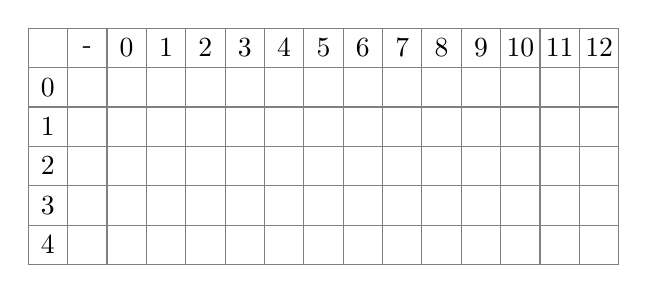
\begin{tikzpicture}
  \draw[step=0.5cm,color=gray] (0,0) grid (7.5,3);
  %% Row 0
  \node at (.75,2.75) {-};
  \node at (1.25,2.75) {0};
  \node at (1.75,2.75) {1};
  \node at (2.25,2.75) {2};
  \node at (2.75,2.75) {3};
  \node at (3.25,2.75) {4};
  \node at (3.75,2.75) {5};
  \node at (4.25,2.75) {6};
  \node at (4.75,2.75) {7};
  \node at (5.25,2.75) {8};
  \node at (5.75,2.75) {9};
  \node at (6.25,2.75) {10};
  \node at (6.75,2.75) {11};
  \node at (7.25,2.75) {12};
  %% Column 0
  \node at (.25,2.25) {0};
  \node at (.25,1.75) {1};
  \node at (.25,1.25) {2};
  \node at (.25,.75) {3};
  \node at (.25,.25) {4};
  \end{tikzpicture}\bigskip
  \end{center}


\end{frame}

\subsection{Coin Change}
\begin{frame}[fragile]{Classical DP -- The Coin Change Problem (CC)}{Problem Summary}
  You are given a target value $V$, and a set $A$ of coin sizes. You have to find the smallest sequence of coins (with repetition) that adds to $V$.
  \bigskip

Example:
\begin{verbatim}
V = 7
A = {1, 3, 4, 5}
  S_0 = { 1, 1, 1, 1, 3}
  S_1 = { 5, 1, 1}
  S_2 = { 3, 3, 1}
  S_3 = { 4, 3}
\end{verbatim}

The best solution is $S_3$.\bigskip

{\bf QUIZ}:
\begin{itemize}
  \item How do you solve this by complete search?
  \item What is the DP Table and Transition?
\end{itemize}
\end{frame}

\begin{frame}[fragile]
  \frametitle{Complete Search for Coin Change}

  We can build a recursive search using the following recurrence on the number of coins $N$ necessary for a given value $V$:
  \[N(V) = 1 + N(V-\text{ size of coin})\]

  \begin{block}{Recursive Complete Search}
    {\smaller
\begin{verbatim}
coins(V):                           // Number of coins for value V:
   if V == 0: return 0              // 0 coins for value 0
   if V < 0:  return MAX_INT        // Can't satisfy for this value
   min = INF                        // Minimum number of coins
   for i in (coins):                // Test each coin
      t = 1 + change(value - A[i])
      if (t < min): min = t
   return t
\end{verbatim}
  }
  \end{block}
\end{frame}

\begin{frame}[fragile]{DP for Coin Change}
  \begin{itemize}
    \item Implementing a Top-down DP should be easy for you now;
    \item Let's make a Bottom-UP DP for practice.
    \item For Bottom-UP DP, it is easier to use a table indexed on COINS
  \end{itemize}

\begin{block}{Bottom-UP DP}
  {\smaller
\begin{verbatim}
boolean DP[c][v] = FALSE;     // Can we reach v with c coins?

i = 0; DP[0][0] = TRUE;       // Start condition
while (TRUE):
  i+=1; possible = FALSE      // Start the loop
  for j = 0 to V:
    if (DP[i-1][j]):          // For each reachable value of V
      possible = TRUE         // We can continue
      if (j == V): return c-1 // Found a solution, go back!
      for k in (coins):       // update all coins
        DP[i][j+k] = TRUE     // Mark new reachable values
  if (!possible): return -1   // No solution found
\end{verbatim}}
\end{block}
\end{frame}

\begin{frame}[fragile]{DP for Coin Change}{Simulation}
\begin{verbatim}
V = 7
A = {1, 3, 4, 5}
\end{verbatim}

\begin{center}
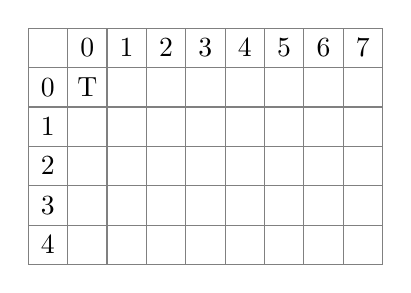
\begin{tikzpicture}
\draw[step=0.5cm,color=gray] (0,0) grid (4.5,3);
%% Row 0
\node at (.75,2.75) {0};
\node at (1.25,2.75) {1};
\node at (1.75,2.75) {2};
\node at (2.25,2.75) {3};
\node at (2.75,2.75) {4};
\node at (3.25,2.75) {5};
\node at (3.75,2.75) {6};
\node at (4.25,2.75) {7};
%% Column 0
\node at (.25,2.25) {0};
\node at (.25,1.75) {1};
\node at (.25,1.25) {2};
\node at (.25,.75) {3};
\node at (.25,.25) {4};
%% Starting Value
\node at (.75,2.25) {T};
\end{tikzpicture}\bigskip
\end{center}
\bigskip

It is interesting to note that the calculation of row $i$ depends only on row $i-1$. Using this information, you can implement the program with a much smaller table.

\end{frame}

%\subsection{Travelling Salesman Problem}
%\begin{frame}
%  \frametitle{Classical DP -- Travelling Salesman Problem}
%
%  We will talk about TSP with DP Next Class!
%\end{frame}

%%%%%%%%%%%%%%%%%%%%%%%%%%%%%%%
% Travelling Salesman Problem (bitmask again)
%% Travelling Salesman Problem (TSP)
% State: tsp(pos,bitmask)
% Transition:
%   Each visited city is a bit in the bitmask
%   - if every city has been visited: tsp(pos, 2^n -1) = dist[pos][0] (back to the start with 0 cities)
%   - Else, try visiting unvisited cities one by one
%   - tsp(pos,bitmask) = min (dist[pos][nxt] + tsp(nxt,bitmask|1<<nt))) for every nxt != pos,
%                                                                           and nxt not visited
%                                                                           bitmask & 1<<nxt == 0

\section{Conclusion}
\begin{frame}
   \frametitle{Summary}

   Dynamic Programming is a search technique that uses memoization to {\bf avoid recalculation overlapping partial solutions}.\bigskip

   There are two main types of solutions:
   \begin{itemize}
   \item \alert{Top-down DP}: Add memory to a recursive full search;
   \item \alert{Bottom-up DP}: Fill the DP table using a for loop;
   \end{itemize}
   \bigskip

   To create a DP, you need to decide the {\bf DP table} and the {\bf Transition rules}.
   \bigskip

   \begin{block}{}
     DP problems are very common in programming competitions. If you are good at DP, you will be able to get a good (but not best) rank in several contests.
   \end{block}
\end{frame}

% \begin{frame}
%    \frametitle{Read more about DP}
%    \begin{itemize}
%       \item \url{http://people.csail.mit.edu/bdean/6.046/dp/}
%       \item \url{http://community.topcoder.com/tc?module=Static&d1=tutorials&d2=dynProg}
%    \end{itemize}
% \end{frame}

% \subsection{Problem Discussion}
%
% \begin{frame}
%    \frametitle{Problem Discussion -- At a Glance}
%    \begin{itemize}
%    \item Wedding Shopping -- Explained in Class
%    \item Jill Rides Again -- Range Sum (1D)
%    \item Largest Submatrix -- Range Sum (2D)
%    \item Is Bigger Smarter? -- Longest Increasing Subsequence
%    \item Murcia's Skyline -- Longest Increasing Subsequence
%    \item Trouble of 13 Dots -- 0-1 Knapsack
%    \item Exact Change -- Coin Change
%    \item Unidirectional TSP -- Pathfinding
%    \end{itemize}
% \end{frame}
%
% % \begin{frame}
% %   \frametitle{Problem Hints}
% %
% %   \begin{itemize}
% %   \item Wedding Shopping
% %   \item Jill Rides Again (Range Sum (1D))
% %   \end{itemize}
% %
% %   \vfill
% %   Discussed during class -- just apply the algorithm!
% % \end{frame}
%
% \begin{frame}
%   \frametitle{Problem Hints}
%
%   \begin{block}{Largest Submatrix}
%     Find the largest patch of {\bf ones} inside a matrix of 1s and 0s.
%   \end{block}
%   \bigskip
%
%   Hints:
%   \begin{itemize}
%   \item Do a range sum to find the rectangle with biggest
%     sum (biggest number of 1).
%   \item {\bf Key Idea}: How do you avoid adding zeroes?
%   \end{itemize}
%   \bigskip
%
%   This kind of problem sometimes appears as the initial part of a more complex problem, to \alert{calculate valid territory}.
% \end{frame}
%
% \begin{frame}
%   \frametitle{Problem Hints}
%
%   \begin{block}{Is bigger Smarter?}
%     You have the "weight" and "intelligence" value of a set of elephants. Find the largest subset where:
%     \begin{itemize}
%     \item A - Intelligence is decreasing, and;
%     \item B - Weight is increasing
%     \end{itemize}
%   \end{block}
%   \bigskip
%
%   Hints:
%   \begin{itemize}
%   \item Think about "Dragon of Loowater" from last lesson.
%   \end{itemize}
% \end{frame}
%
% \begin{frame}
%   \frametitle{Problem Hints}
%   \begin{block}{Murcia Skyline}
%     Compare the size of the Longest {\bf Increasing} skyline and the longest {\bf Decreasing} skyline.
%   \end{block}
%   \bigskip
%
%   Hints:
%   \begin{itemize}
%   \item "Longest Increasing Subsequence" in this problem is modified by the {\bf building width}.
%   \end{itemize}
% \end{frame}
%
% \begin{frame}
%   \frametitle{Problem Hints}
%   \begin{block}{Trouble of 13 dots}
%     Find the subset of items that:
%     \begin{itemize}
%     \item Mazimize flavor;
%     \item Is inside the price budget; You can get a discount;
%     \end{itemize}
%   \end{block}
%
%   \bigskip
%
%   Hints
%   \begin{itemize}
%   \item 1-0 knapsack problem:
%   \item Be careful with special rule: {\bf the knapsack change size if price > 2000!}
%   \end{itemize}
% \end{frame}
%
% \begin{frame}
%   \frametitle{Problem Hints}
%   \begin{block}{Exact Change}
%     Find the smallest amount of overpay that you can do, with the
%     smallest number of coins.
%   \end{block}
%
%   \bigskip
%   Hints:
%   \begin{itemize}
%   \item Variation of the Coin Change problem discussed in Class;
%   \item Calculate all possible changes above the desired value, and find the smallest;
%   \item Order by smallest number of coins necessary;
%   \item Bottom Up algorithm is probably best;
%   \end{itemize}
% \end{frame}
%
% \begin{frame}
%   \frametitle{Problem Hints 6}
%   \begin{block}{Unidirectional TSP}
%     Find the minimal path from left to right. Up and down are connected!
%   \end{block}
%
%   \bigskip
%
%   \begin{itemize}
%   \item Very similar to the ``apple robot'' problem;
%   \item Note that when two paths have the same weight, the smaller index is best!
%   \end{itemize}
% \end{frame}

%\subsection{Extra}
%\begin{frame}
%  \frametitle{Extra -- ICPC Call to Arms!}

%  {\smaller
%  If you can solve complete search and DP problems quickly, \alert{you
%  probably can reach top 50\%} at the ICPC first round. Why not try it this year?
%
%  \begin{block}{ICPC team registration -- Deadline 06/10 -- Contest 06/23}
%    Send message to caranha@cs.tsukuba.ac.jp with the following information:
%    \begin{itemize}
%    \item Team Name -- roman letters, numbers and symbols
%    \item Team Member 1 -- Name (letters), Name (japanese), e-mail, student ID
%    \item Team Member 2 -- Name (letters), Name (japanese), e-mail, student ID
%    \item Team Member 3 -- Name (letters), Name (japanese), e-mail, student ID
%    \end{itemize}
%  \end{block}}


%  {\tiny
%  \begin{itemize}
%  \item Japan 1st Round contest 2011 --\\
%    \url{http://ichyo.jp/aoj-icpc/?source4=0&source2=0&source3=0&source1=1&year_max=2011&year_min=2011}
%  \item Japan 1st Round contest 2012 --\\
%    \url{http://ichyo.jp/aoj-icpc/?source4=0&source2=0&source3=0&source1=1&year_max=2012&year_min=2012}
%  \item Japan 1st Round contest 2013 --\\
%    \url{http://ichyo.jp/aoj-icpc/?source4=0&source2=0&source3=0&source1=1&year_max=2013&year_min=2013}
%  \item Japan 1st Round contest 2014 --\\
%    \url{http://ichyo.jp/aoj-icpc/?source4=0&source2=0&source3=0&source1=1&year_max=2014&year_min=2014}
%  \end{itemize}}
%\end{frame}
%\end{document}


%%%%%%%%%%%%%%%%%%%%%%%%%%%%%%%%%%%%%%%%%%%%%%%%%%%%
\section{Backmatter}
\begin{frame}{About these Slides}
  These slides were made by Claus Aranha, 2020. You are welcome to copy, re-use and modify this material.
  \bigskip

  Individual images in some slides might have been made by other
  authors. Please see the references in each slide for those cases.
\end{frame}

\begin{frame}[allowframebreaks]{Image Credits}
  \printnotes
\end{frame}

\end{CJK}
\end{document}
